% ==================================================================

\chapter{Introductie tot Elektrische Machines}
% Inhoud volgt
Een typische toepassing van elektrische machines is alles dat te maken heeft met
aandrijving.
Elektrische motoren kunnen klein tot groot zijn en generatoren bestaan dus ook en worden
gebruikt voor het genereren van elektriciteit, deze kunnen ook klein of groot zijn.
(Kan tot 5MW, dit is een windturbine).
\newline
Motoren zijn energieomzetters (\textbf{convertors}) die \textit{elektrische energie
omzetten tot mechanische energie} en generatoren zijn energieomzetters die
\textit{mechanische energie omzetten tot elektrische energie}.
In deze cursus wordt vooral de focus op roterende motoren gelegd, niet op lineaire.

\begin{figure}[H]
  \centering
  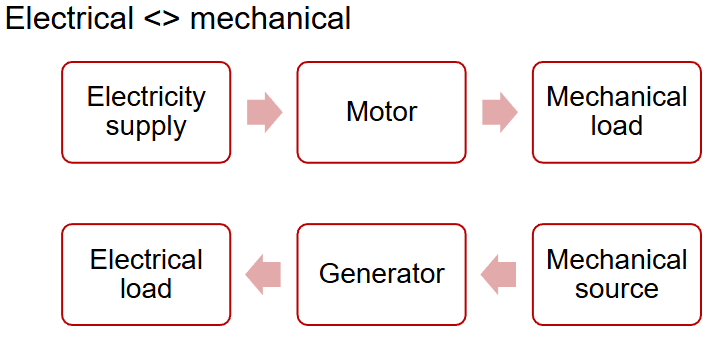
\includegraphics[width=0.5\textwidth]{assets/energieconversiemotorengenerator.png}
  \caption{Motor en generator energieconversie}
  \label{fig:energieconversiemotorengenerator.png}
 \end{figure}

Vaak zijn wel nog extra omvormers nodig voor de perfecte werking zoals \textit{Power
eletronics} die bevoorbeeld eerst de spanning van een generator omvormt naar een andere
spanning die nodig is voor de motor.
En een tandwielkast kan ook nodig zijn om de snelheid van de motor aan te passen aan de
toepassing.
Hier gaan we niet dieper op in.
Ook wordt vaak nog een controller gebruikt om de motor op een goeie manier te laten
werken, dit is dus eigelijk \textit{terugkoppeling} (feedback).

\begin{figure}[H]
  \centering
  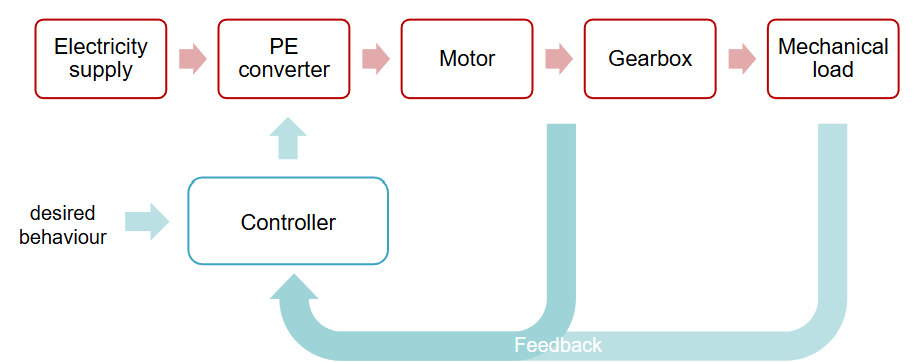
\includegraphics[width=0.6\textwidth]{assets/omzettingmetfeedback.png}
  \caption{Energieomzetting met feedback}
  \label{fig:omzettingmetfeedback.png}
 \end{figure}

Het vak gaat hier vooral over welk effect op de motor welk gedrag heeft op de uitgang (de
'mechanical load')

\section{Karakteristieken}

\subsection{Motor-last interactie}
Een motor moet dus een kracht leveren om deze beweging te realiseren.
Met de wet van Newton kunnen we dit beschrijven en dus bepalen hoe hard de motor een
object versnelt:
\begin{align*}
    \sum = F_{motor} - F_{load} = m \cdot a
\end{align*}
Hierbij is $F_{motor}$ de aandrijfkracht die de motor levert, $F_{load}$ de kracht die de
last uitoefent op de motor (dus de 'tegenwerkende kracht van de belasting'), $m$ de massa
van het object en $a$ de versnelling.
Op een bepaald moment gaat de motor een constante snelheid bereiken (\textit{'Steady
state'}), de versnelling wordt hier dan 0 en de krachten zijn in evenwicht.
De motor levert dan een kracht die gelijk is aan de kracht van de last.
De motor moet dus een koppel leveren dat gelijk is aan het koppel van de last.
Het koppel van de motor wordt bepaald door de elektrische eigenschappen van de motor en de
spanning die erop wordt gezet.
Het koppel van de last wordt bepaald door de mechanische eigenschappen van de last en de
snelheid waarmee deze beweegt.
Volgend voorbeeld wordt aan bord in de les gemaakt:

\subsubsection{Voorbeeld Trein}
\textit{Een trein rijd met een constante snelheid van 40 km/h.
De trein heeft een massa van 40 ton en de wrijving van de rails is 4 kN.
Rijden vermeerderd die kracht met 20 kN in de positieve richting van de beweging, dit is
dus de motorkracht.
Wat is op dit moment de versnelling en wat gebeurt er daarna?}
\newline
We kunnen hier de wet van Newton toepassen:
\begin{align*}
    \sum = F_{motor} - F_{load} = m \cdot a
\end{align*}
We weten dat de massa van de trein 40 ton is, dit is 40000 kg.
De kracht van de motor is 20 kN en de kracht van de last is 4 kN.
We kunnen dit invullen in de vergelijking:
\begin{align*}
    20 kN - 4 kN = 40000 kg \cdot a
\end{align*}
\begin{align*}
    16 kN = 40000 kg \cdot a
\end{align*}
\begin{align*}
    a = \frac{16 kN}{40000 kg} = 0.4 m/s^2
\end{align*}

\subsubsection{Voorbeeld fiets}
Hier wordt een fiets gebruikt als voorbeeld, de proff geeft hier simpelweg het volgende:
\begin{align*}
    F_{motor} = 40 - 4 \cdot v
\end{align*}
Met motor de kracht op een pedaal door een persoon
\begin{align*}
  F_{load} = 10 + 0,4 \cdot v^2
\end{align*}
Met load de tegenwerkende kracht op een pedaal door bvb.
de weg, fiets, mechanica van de fiets, etc.
\newline
Hier wordt gevraagd achter de regimesnelheid van de fiets (Steady State) (dus wanneer
$a = 0$).
\begin{align*}
    F_{motor} = F_{load}
\end{align*}
\begin{align*}
    40 - 4 \cdot v = 10 + 0,4 \cdot v^2
\end{align*}
Dit geeft v = 5 m/s.
Deze 2 krachten plotten in functie van de snelheid geeft een mooi overzicht van de
krachten en hun snijpunt:

\begin{figure}[H]
  \centering
  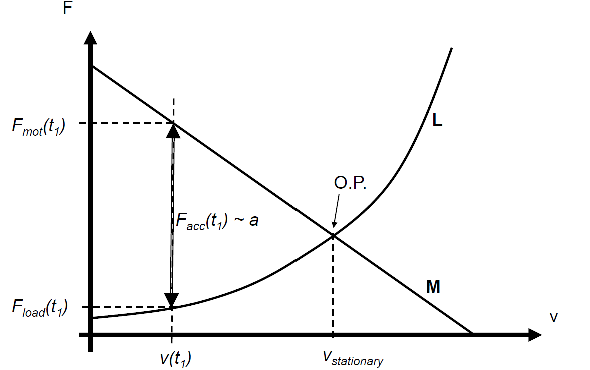
\includegraphics[width=0.6\textwidth]{assets/karakteristiekmetwerkingspunt.png}
  \caption{Krachten ifv snelheid}
  \label{fig:karakteristiekmetwerkingspunt.png}
 \end{figure}

O.P.
is het \textbf{werkingspunt} (Operating Point), het is dus hier dat dat evenwicht is.
Een \textbf{karakteristiek} is een grafiek/verzameling van grafieken die de relatie tussen
2 grootheden weergeeft alsook de werkingspunten.
Een voorbeeld is de koppel-toerentalkarakteristiek van een motor.

\subsection{Werkingspunt}
Dus een werkingspunt is een evenwicht punt van de motor en de last.
Voor een koppeltoerentalkarakteristiek zien we deze weergegeven als punt 1 en punt 2 in
onderstaande figuur.
Het zijn hier dus punten waar in dit geval de koppels van de last gelijk zijn aan die van
de motor.
Echter hebben we ook nog \textbf{stabiele} en \textbf{onstabiele} werkingspunten.
Een stabiel werkingspunt is een werkingspunt waar bij afwijking van dat werkingspunt de
motor en last elkaar nog gaan corrigeren en dus de motor terugbrengen naar dat
werkingspunt.
Neem als afwijking een snelheidsfout in punt 1, het toerental zal dalen tot punt 1', nu
heeft de motor niet genoeg koppel meer om de last te dragen dus kan het niet terug
versnellen tot punt 1, dit is dus een instabiel werkingspunt.
Bij een snelheidsfout rond punt 2 is er oftewel genoeg koppel om te versnellen (punt 2')
oftewel vertraagt de motor gewoon terug tot punt 2 als er een snelheidsfout tot punt 2''
was.

\begin{figure}[H]
  \centering
  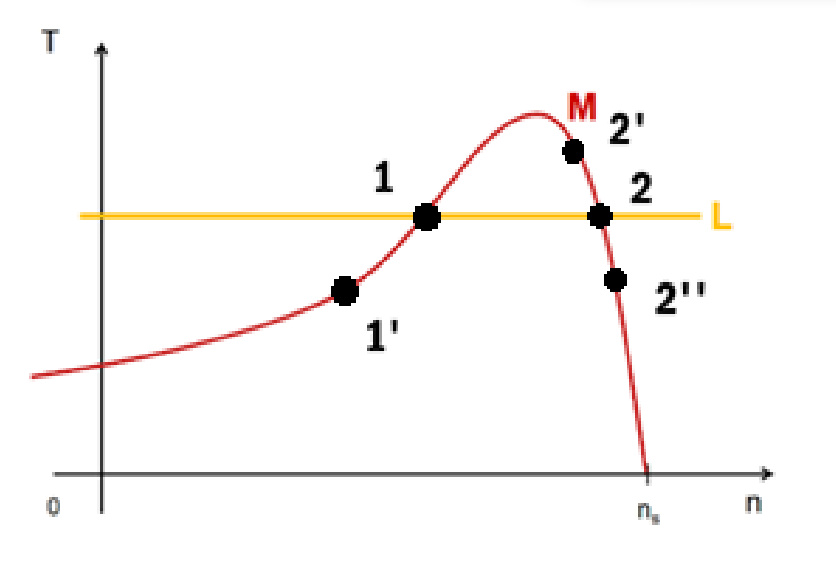
\includegraphics[width=0.6\textwidth]{assets/stabielenonstabielewerkingspuntenopTn.png}
  \caption{T-n karakteristiek motor en last met stabiele en onstabiele werkingspunten}
  \label{fig:stabielenonstabielewerkingspuntenopTn.png}
 \end{figure}

\subsection{Typische last karakteristieken}
In de les worden een paar typische lastkarakteristieken besproken:

\begin{figure}[H]
  \centering
  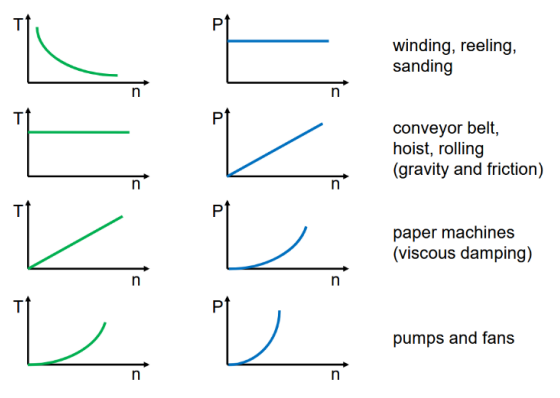
\includegraphics[width=0.4\textwidth]{assets/lastkarakteristieken.png}
  \caption{Typische lastkarakteristieken}
  \label{fig:lastkarakteristieken.png}
 \end{figure}

Veel diepgaand wordt het hier niet gesproken, gewoon dat die bovenste grafiek van
'winding, reeling, sanding' typisch een karakteristiek is van een geval waar de diameter
steeds veranderd, hier is een constant vermogen, wat normaal niet vaak het geval is, de
T-n ziet er dan hyperbolisch uit.
En de 2de bovenste, die met het constante koppel, is de meest voorkomende karakteristiek,
hierbij treedt voornamelijk zwaartekracht en wrijving op wat dus de meest voorkomende
krachten zijn bij een machine.

\subsection{4 kwadrantoperaties}
Een elektrisch toestel (motor/generator) kan in 4 kwadranten werken, dit is afhankelijk
van de richting van het koppel en de richting van de snelheid.
In \textbf{kwadrant 1} werkt de motor als motor, dit is de \textit{normale werking}, het
\textit{koppel is in dezelfde richting als de rotatie}, in \textbf{kwadrant 2} werkt de
motor als generator, het \textit{koppel is in tegengestelde richting van de draairichting}
(hier is het koppel positief) kwadrant 2 is dus remmend, in \textbf{kwadrant 3} werkt de
motor als motor maar in tegengestelde richting en in \textbf{kwadrant 4} werkt de motor
als generator maar in tegengestelde richting, het is hier dus een negatief koppel.
Dit wordt vaak gebruikt bij elektrische voertuigen, waarbij de motor kan remmen
\textbf{(regeneratief remmen)} en dus energie terug kan leveren aan de batterij.

\begin{figure}[H]
  \centering
  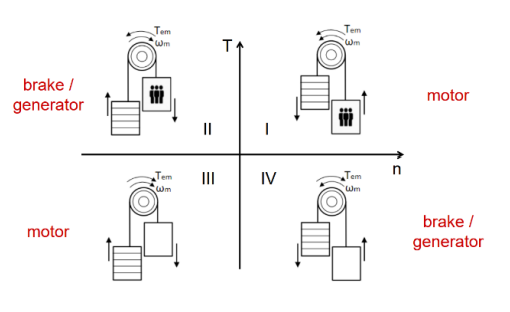
\includegraphics[width=0.5\textwidth]{assets/4kwadrantoperaties.png}
  \caption{4 kwadrantoperaties}
  \label{fig:4kwadrantoperaties.png}
 \end{figure}

\subsection{Nominale waardes}
De juiste motor voor je toepassing kiezen ga je doen afhankelijk van de eigenschappen van
die motor:
bvb.
zoveel kW bij zoveel snelheid, motor selectie wordt dus met een catalogus gedaan, het
toont dus eigelijk de waardes van de kenplaten van de motoren.
Op zo een kenplaat staan \textbf{nominale waardes}, dit zijn de waardes waarvoor een motor
ontwikkeld is om rond te werken.
Dus eigelijk wat je continu kan doen.
Indien je hoger dan deze nominale waardes gaat (dit kan) ga je rapper opwarmen, dit is
niet gewenst want is slecht voor de motor dus je kan dit niet continu doen.
Eigelijk zijn nominale waardes dus een \textit{thermische grens}.
Belangrijk te weten is dus dat het vermogen van de motor niet constant is, het vermogen
dat op de kentekenplaat staat is het nominale vermogen, en het vermogen bij gebruik kan
anders zijn.
Kleine machines wijken het meeste af (van nominale waardes voor snelheid bvb.), we zeggen
dat ze een slechter \textbf{rendement} hebben.

Het rendement is eigelijk de \textbf{efficiëntie} van de motor, het is de verhouding van
het nuttige vermogen dat uit de motor komt en het vermogen dat in de motor gaat.
Het rendement is dus een maat voor hoe goed de motor energie omzet in nuttig werk.
Het rendement wordt vaak uitgedrukt in procenten en kan berekend worden met de volgende
formule:
\begin{align*}
    \eta = \frac{P_{out}}{P_{in}} \cdot 100\%
\end{align*}
Waarbij $\eta$ het rendement is, $P_{out}$ het nuttige vermogen dat uit de motor komt
(eigelijk het mechanische vermogen) en $P_{in}$ het vermogen dat in de motor gaat (dus het
elektrisch vermogen).

\begin{warningbox}[Het rendement en de arbeidsfactor zijn niet hetzelfde!]
    De arbeidsfactor bereken je met de formule:
    \begin{align*}
        \cos(\varphi) = \frac{P_{act}}{P_{schijn}}
    \end{align*}
    Numeriek lijken ze op elkaar maar ze zijn niet hetzelfde.
    Het rendement is een maat voor hoe goed de motor energie omzet in nuttig werk, terwijl
    de arbeidsfactor een maat is voor hoe goed de motor het elektrische vermogen gebruikt.
    Ze betekenen dus iets totaal anders.
\end{warningbox}

\section{Constructie}

\subsection{Motortypes}
Er zijn verschillende motortypes, vooral geclassificeerd op basis van hun voeding:

\begin{itemize}
 \item \textbf{AC Drie fasig}:
 Dit wordt vooral in de industrie gebruikt, deze hebben een beetje meer koper nodig dan
 een 1 fasige motor maar kunnen veel meer vermogen leveren.
 \item \textbf{AC Een fasig}: Dit wordt vooral in huishoudtoepassingen gebruikt.
 \item \textbf{DC}:
 Deze worden vooral gebruikt in voertuigen, zoals elektrische auto's, treinen, trams, etc.
 Ze hebben een goede regelbaarheid van het koppel en de snelheid.
 \item \textbf{Power Electronics}:
 (Op deze gingen we niet dieper in, het hoort wel bij deze motortypes)
\end{itemize}

Tussen de verschillende AC machines zijn er ook nog verschillende types, zoals
\textbf{synchrone} (\textbf{Inductiemachine}) en \textbf{asynchrone} machines.
Deze zien we later nog.
Er zijn ook nog andere verschillende types die we niet echt bezien $\cdots$

Ook is er nog onderverdeling tussen Motoren en Generatoren.

\subsection{Constructie}
Een typische motor bestaat uit meerdere componenten die we aangeduid zien in de volgende
figuur:

\begin{figure}[H]
  \centering
  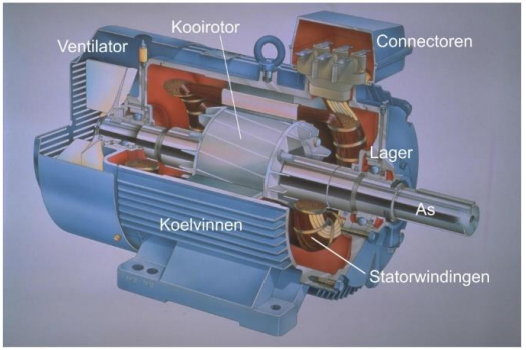
\includegraphics[width=0.6\textwidth]{assets/constructiemotor.png}
  \caption{Motor constructie inductiemachine}
  \label{fig:constructiemotor.png}
 \end{figure}

\begin{itemize}
 \item \textbf{Ventilator}:
 Dit dient om de motor te koelen, vooral belangrijk om de 'lak' / 'isolatie' van de
 wikkelingen niet te doen smelten.
 \item \textbf{Behuizing}:
 Dit dient om de motor te beschermen tegen stof, vuil, vocht, etc.
 Maar ook belangrijk om warmte af te voeren, daarom staan er ook vaak \textbf{koelvinnen}
 op de behuizing.
 Het moet dus belangrijke thermische eigenschappen hebben en bestaat dus uit
 \textbf{gietijzer}.
 \item \textbf{Rotor}:
 Dit is het draaiende deel van de motor, dat werkt op basis van elektromagnetisme.
 Het bestaat uit wikkelingen die door elektriciteit worden aangedreven.
 Hier zien we een \textbf{kooirotor} (het is dus een inductie motor), de stroom gaat dus
 door \textbf{Aluminium} (in een DC motor is dit koper).
 \item \textbf{Stator}:
 Dit is het stilstaande deel van de motor \textit{hier} (bij sommige motors is dit
 omgekeerd).
 Het zit binnenin de behuizing en bestaat uit \textbf{statorijzer}
 (\textit{Siliciumstaal}, dit is goed om magnetische veldlijnen te geleiden) (de kern) en
 \textbf{statorwikkelingen} (\textit{koper}) die in de gleuven van de kern liggen.
 \item \textbf{As/Shaft}:
 Dit is de as die de rotor aandrijft en het mechanische vermogen levert aan de belasting.
 Het is meestal gemaakt van \textbf{staal} en is verbonden met de rotor.
 \item \textbf{Lager}: Ondersteunt de as en zorgt dat deze soepel kan draaien.
 \item \textbf{Connectoren}:
 Deze dienen om de spanning aan te sluiten.
 In de meeste gevallen kunnen we hier ook kiezen of we de motor in ster of driehoek
 zetten.
\end{itemize}

\subsection{Magnetische Permeabiliteit}
Door het feit dat er een magnetisch veld wordt opgewekt in de motor, is het belangrijk dat
de materialen die gebruikt worden een hoge magnetische permeabiliteit hebben.
Dit betekent dat ze goed in staat zijn om magnetische veldlijnen te geleiden.
Siliciumstaal wordt vaak gebruikt voor de kern van de stator en rotor omdat het een hoge
permeabiliteit heeft en ook goed bestand is tegen verzadiging.
Verzading treedt op wanneer het materiaal niet meer in staat is om extra magnetische flux
te geleiden, wat kan leiden tot verlies van efficiëntie en warmteontwikkeling.
Dat gietijzer zou enorme verliezen geven dus, daarom is het als behuizing prima want het
is sterk en voert warmte goed af.

We zijn dus geïnteresseerd in ferromagnetische materialen, als we kijken naar de
onderstaande figuur kunnen we zien hoe magnetische velden in een materiaal gealigneerd
kunnen zijn:

\begin{figure}[H]
  \centering
  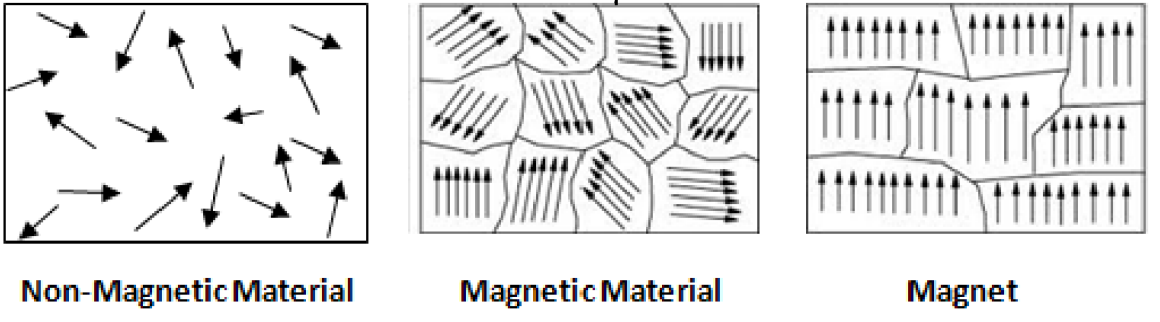
\includegraphics[width=0.8\textwidth]{assets/allignerenmagnetische-velden.png}
  \caption{Alligneren van de magnetische velden}
  \label{fig:allignerenmagnetische velden.png}
 \end{figure}

In de linkse figuur een niet ferro-magnetisch materiaal, alle pijlen zijn hier in alle
richtingen gealigneerd (dit is op atomair niveau), geen netto magnetisch veld.
In het midden een magnetisch materiaal hier zijn pijlen in groepjes verdeeld en elk
groepje heeft een netto magnetisch veld maar het totaal geheel niet, dit kan wel
gemagnetiseerd worden door een extern magnetisch veld.
In de rechtse figuur is het materiaal volledig gealigneerd, dit is een permanent magneet.
Het materiaal heeft hier een hoge permeabiliteit en kan dus goed magnetische flux
geleiden.
Doordat deze allemaal in dezelfde richting staan, is dit een sterk veld.

Het is dan dit fenomeen dat de permeabiliteit van een materiaal bepaalt, hoe beter de
atomen in het materiaal zich kunnen aligeneren met het externe veld, hoe hoger de
permeabiliteit.

\begin{figure}[H]
  \centering
  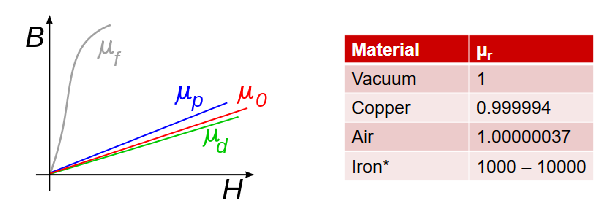
\includegraphics[width=0.8\textwidth]{assets/magnetischepermeabiliteit.png}
  \caption{Magnetische permeabiliteit van verschillende materialen (µ)}
  \label{fig:magnetischepermeabiliteit.png}
 \end{figure}

Hier is B de magnetische fluxdichtheid, H de magnetische veldsterkte en \textbf{µ de
magnetische permeabiliteit}.
De permeabiliteit van een materiaal is dus een maat voor hoe goed het materiaal in staat
is om magnetische flux te geleiden.
De helling zegt \textit{'hoeveel stroom je nodig hebt voor hoeveel magnetisch veld'}.
En met dat magnetisch veld maak je dus de krachten die de motor doen draaien.

Nog iets belangrijks is de \textbf{hysteresis lus}, dit is een grafiek die de relatie
tussen B en H weergeeft.
Het toont ons echter ook de \textbf{remanente inductie}, dit is de magnetische flux die in
het materiaal blijft nadat het externe veld is verwijderd.
Dit is belangrijk omdat het kan leiden tot verlies van efficiëntie en warmteontwikkeling
in de motor.
Het toont ook de \textbf{coerciviteit}, dit is de kracht die nodig is om het materiaal te
demagnetiseren (dus hoe hard we de veldsterkte moeten tegenwerken zodat de magnetische
flux terug nul is).
Materialen met een hoge coerciviteit zijn beter bestand tegen verzadiging en kunnen dus
beter presteren in een motor.

\begin{figure}[H]
  \centering
  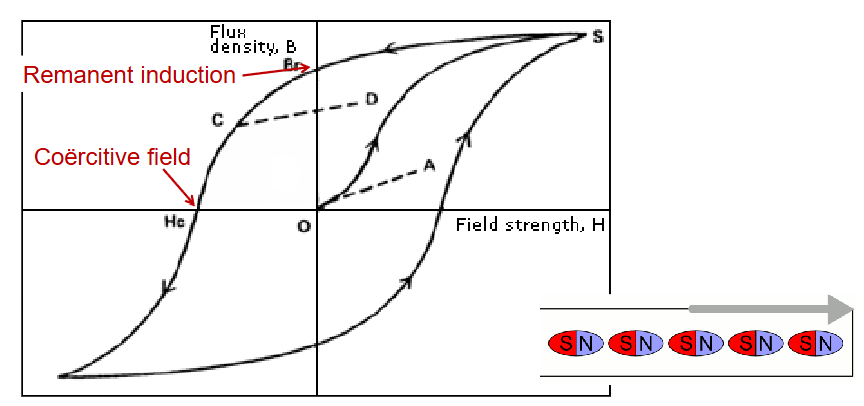
\includegraphics[width=0.5\textwidth]{assets/hysteresislus.png}
  \caption{Hysteresislus van een magnetisch materiaal}
  \label{fig:hysteresislus.png}
 \end{figure}

Een materiaal met een \textbf{kleine lus} noemen we een \textbf{zacht magnetisch
materiaal}, dit is goed voor motoren.
Een materiaal met een \textbf{grote lus} noemen we een \textbf{hard magnetisch materiaal},
dit is goed voor permanente magneten.
De stator moet dus uit zo een zacht materiaal gemaakt worden aangezien dit op AC 50 keer
de lus doet (50 Hz), dus dan hebben we minder verliezen.
De rotor die volgt gewoon en dit kan met permanente magneten gedaan worden (kan ook met
wikkelingen gedaan worden zoals de stator), dit is dan dus met een hard magnetisch
materiaal (heeft een brede lus, magnetisch veld blijft, brede lus nodig dus).

\begin{figure}[H]
  \centering
  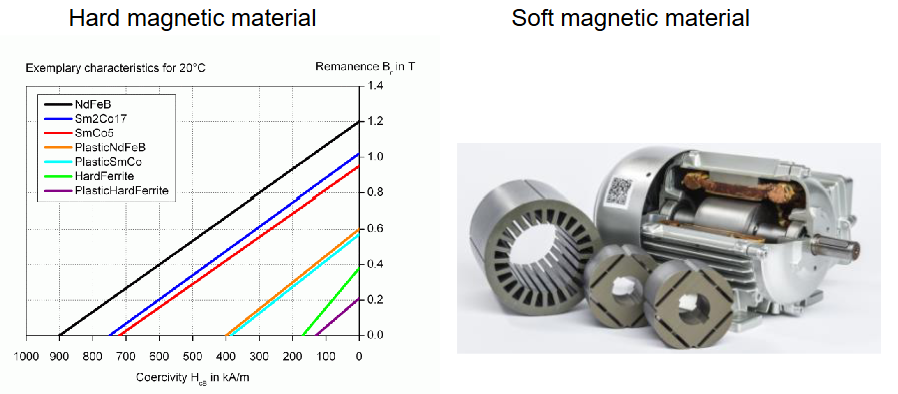
\includegraphics[width=0.8\textwidth]{assets/hardenzachtmagnmateriaak.png}
  \caption{Hard en zacht magnetisch materiaal}
  \label{fig:hardenzachtmagnmateriaak.png}
 \end{figure}

\subsection{Stator Constructie}
Dus de stator is het 'statische' deel van de motor, het bestaat dus uit die siliciumstaal
kern met gleuven in, het heeft dus eigelijk 'statortanden', hierin bevestigen zich de
statorwikkelingen.
De statorwikkelingen zijn meestal van koper en zijn geïsoleerd om kortsluiting te
voorkomen.
De wikkelingen zijn zo geplaatst dat ze een magnetisch veld opwekken wanneer er stroom
doorheen loopt.
Dit magnetisch veld wisselt van richting afhankelijk van de stroomrichting, wat essentieel
is voor de werking van de motor.

\begin{figure}[H]
  \centering
  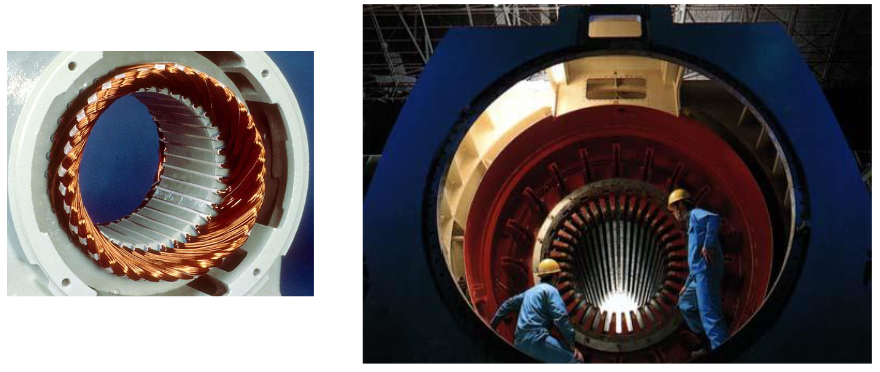
\includegraphics[width=0.6\textwidth]{assets/statorvisueel.png}
  \caption{Stator constructie met statortanden en wikkelingen}
  \label{fig:statorvisueel.png}
 \end{figure}

De wikkelingen kunnen op 2 manieren gewonden worden: 

\begin{itemize}
 \item \textbf{Geconcentreerd}:
 Hier heb je spoelen geconcentreerd rond individuele statortanden, het magnetisch veld
 opgewekt is dus eigelijk blokvormig, dus sterk recht per tand en niet zo mooi naast de
 tanden, het gevolg is een veld met veel harmonischen.
 Dit is goedkoper door minder koper maar heeft meer verliezen bij gebruik.
 \begin{figure}[H]
   \centering
   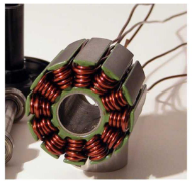
\includegraphics[width=0.4\textwidth]{assets/geconcentreerd.png}
   \caption{Geconcentreerde wikkelingen}
   \label{fig:geconcentreerd.png}
  \end{figure}
 \item \textbf{Gedistribueerd (verdeelde)}:
 Hier zijn de wikkelingen verdeeld over meerdere statortanden, er kunnen dus meerdere
 wikkelingen per gleuf op elkaar liggen, het magnetisch veld opgewekt is dus veel mooier
 en vloeiender, het gevolg is een veld met minder harmonischen.
 Dit is duurder door meer koper maar heeft minder verliezen bij gebruik.
 \begin{figure}[H]
   \centering
   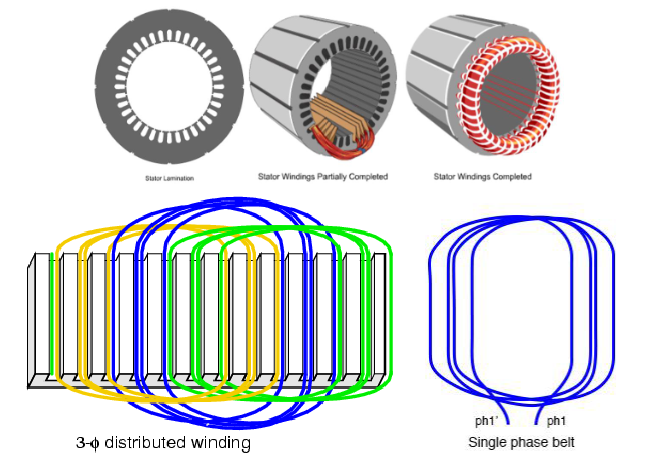
\includegraphics[width=0.6\textwidth]{assets/verdeelde.png}
   \caption{Gedistribueerde wikkelingen}
   \label{fig:verdeelde.png}
  \end{figure}
Meestal worden verdeelde wikkelingen gebruikt.
\end{itemize}

De statorkern zelf wordt in lamellen opgebouwd om wervelstromen te beperken
(jouleverliezen), deze lamellen vormen samen nog steeds de blokvormige statorkern:

\begin{figure}[H]
  \centering
  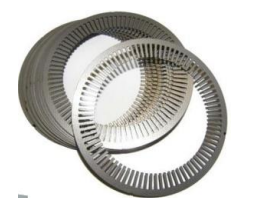
\includegraphics[width=0.4\textwidth]{assets/lamellenstator.png}
  \caption{Lamellen in de statorkern}
  \label{fig:lamellenstator.png}
 \end{figure}

\subsection{Rotor Constructie}
De stator constructie blijft vaak ongeveer hetzelfde maar bij de rotor is dit een ander
verhaal, de constructie \textit{verschilt hier meer per machine/motortype.} Voor
\textbf{de Synchrone machine} kan dit met \textbf{permanente magneten} of met \textbf{DC
wikkelingen} gedaan worden.

\subsubsection{Permanente magneten}
Bij een rotor met permanente magneten zijn de magneten op de rotor bevestigd en zorgen ze
voor een constant magnetisch veld.
Dit type rotor is vaak compacter en efficiënter, maar kan duurder zijn vanwege de kosten
van de permanente magneten.
Hierbij kunnen we ook nog 2 types hebben:

\begin{itemize}
 \item \textbf{Uitspringende polen}:
 Hier heb je wat lucht tussen de polen, de magneten zijn er eigelijk opgeplakt, dit wordt
 het meest in de praktijk gebruikt want geeft een goede regeling (zien we later).
 \item \textbf{Gladde rotor}:
 Hier zijn geen gaten, de rotor is volledig dicht eigelijk, dit heeft als voordeel dat het
 'magnetisch glad' is want dde veldlijnen komen direct ijzer tegen, dit maakt het
 symmetrischer.
\end{itemize}

\begin{figure}[H]
  \centering
  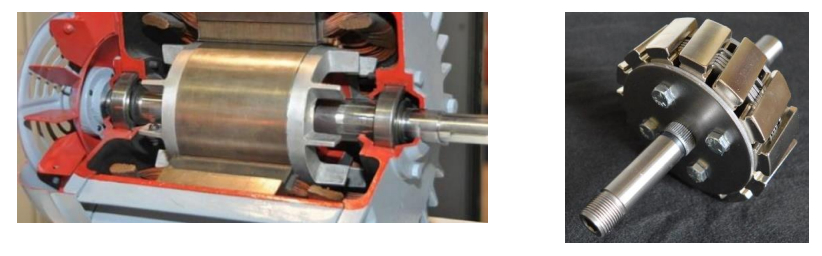
\includegraphics[width=0.8\textwidth]{assets/gladvsuitspringend.png}
  \caption{Gladde vs. uitspringende polen}
  \label{fig:gladvsuitspringend.png}
 \end{figure}

\subsubsection{DC Wikkelingen}
Dit is een rotor die wikkelingen er al op heeft staan en die gevoed worden met een DC-bron
om een soort van permanente magneet te maken.
Om deze constante stroom te voorzien worden \textbf{sleepringen} gebruikt, dit zijn
metalen ringen (meestal koper) waar een \textbf{koolstofborstel} (dit roteert dus niet) op
gedrukt wordt zodat de stroom van de DC-bron hierdoor naar de sleepringen van de rotor kan
gaan.

\begin{figure}[H]
  \centering
  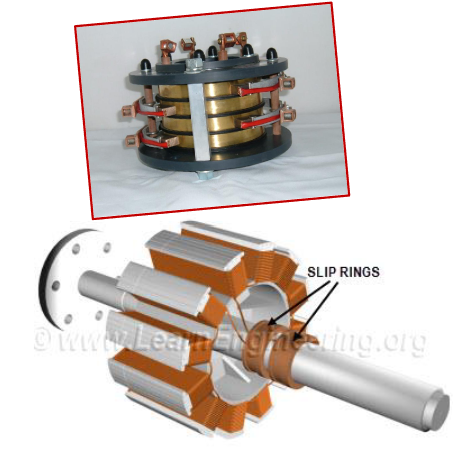
\includegraphics[width=0.4\textwidth]{assets/sleepringen.png}
  \caption{Sleepringen in de rotor}
  \label{fig:sleepringen.png}
 \end{figure}

Bij de \textbf{DC-machine} gebruiken we iets gelijkaardig, namelijk een
\textbf{commutator} bij de constructie van de rotor:

\subsubsection{Commutator}
Het grote verschil met de sleepring hier is dat het onderbrekingen heeft, het wordt dus
eigelijk gebruikt om wikkelingen op de rotor aan en uit te schakelen, dit is nodig om de
stroomrichting in de rotorwikkelingen te veranderen zodat het magnetisch veld van de rotor
altijd in dezelfde richting blijft ten opzichte van de stator.
Dit is essentieel voor de werking van de DC-machine, omdat het ervoor zorgt dat het koppel
constant blijft tijdens de rotatie.
Ook hier worden koolstofborstels tegen geduwd.
Een probleem is wel dat hier vonken kunnen onstaan.

\begin{figure}[H]
  \centering
  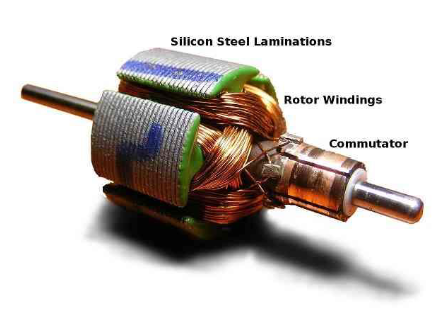
\includegraphics[width=0.4\textwidth]{assets/commutator.png}
  \caption{Commutator in de rotor}
  \label{fig:commutator.png}
 \end{figure}

\subsubsection{Inductiemachine}
Bij de \textbf{inductiemachine} kan de rotor een \textbf{kooirotor} of een
\textbf{wikkelrotor} zijn.
Bij de kooirotor zijn er geen wikkelingen op de rotor, maar geleiders die in een
kooivormige structuur zijn geplaatst.
Dit type rotor is robuuster en veel \textbf{goedkoper}, vooral door het productieproces
want je giet dit gewoon in aluminium, het heeft ook geen sleepringen/commutator en geen
onderhoud nodig, maar heeft minder regelbaarheid dan een wikkelrotor.
Bij de wikkelrotor zijn er wikkelingen op de rotor die via sleepringen en koolstofborstels
worden gevoed, dit geeft meer regelbaarheid maar is duurder en complexer.

\begin{figure}[H]
  \centering
  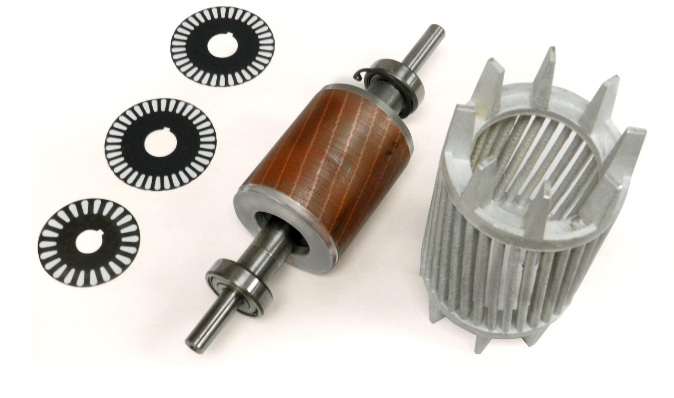
\includegraphics[width=0.5\textwidth]{assets/kooirotor.png}
  \caption{Kooirotor}
  \label{fig:kooirotor.png}
 \end{figure}

\begin{figure}[H]
  \centering
  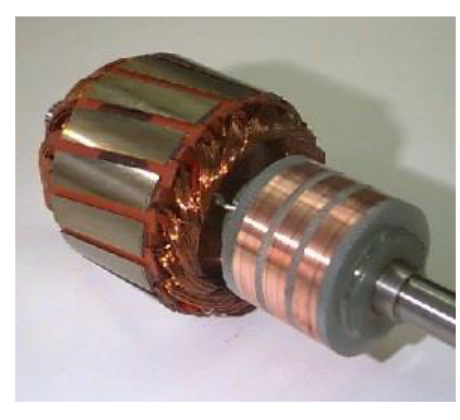
\includegraphics[width=0.4\textwidth]{assets/gewikkelderotor.png}
  \caption{Wikkelrotor}
  \label{fig:gewikkelderotor.png}
 \end{figure}

\newpage
